\pdfminorversion=7
\documentclass[a4paper,fleqn]{cas-sc}

\usepackage[authoryear,longnamesfirst]{natbib}
\usepackage{amsmath}
\usepackage{amssymb}
\usepackage{booktabs}
\usepackage{multirow}
\usepackage{graphicx}
\usepackage{array}
\usepackage{xcolor}
\usepackage{url}
\usepackage{placeins}
\usepackage{float}
\usepackage{tikz}
\usetikzlibrary{arrows.meta,positioning,fit,backgrounds,calc,shapes.geometric}
\hypersetup{hidelinks,hypertexnames=false}
\emergencystretch=2em

% Target journal: Neurocomputing
\newcommand{\tbc}[1]{\textcolor{red}{[TO BE CONFIRMED: #1]}}

\begin{document}
\let\WriteBookmarks\relax
\def\floatpagepagefraction{1}
\def\textpagefraction{.001}

\shorttitle{Directed Ordinal-Token Graphs for DR Grading}
\shortauthors{Zhuang et al.}
\title[mode=title]{Directed Ordinal-Token Graphs for Diffusion-Based Diabetic Retinopathy Grading}

% Verify all author metadata before submission.
\author[aff1]{Shuo Zhuang}
\author[aff1]{Author 2 (TBC)}
\author[aff2]{Corresponding Author (TBC)}
\cormark[1]
% Replace TBC with the verified corresponding-author email before submission.
\ead{TBC}
\cortext[1]{Corresponding author}
\affiliation[aff1]{organization={Department / School / Institution 1 (TBC)},city={City (TBC)},postcode={Postcode (TBC)},state={Province / State (TBC)},country={Country (TBC)}}
\affiliation[aff2]{organization={Department / School / Institution 2 (TBC)},city={City (TBC)},postcode={Postcode (TBC)},state={Province / State (TBC)},country={Country (TBC)}}

\begin{abstract}
Diabetic retinopathy grading depends on subtle changes in lesion burden. Standard multiclass prediction does not explicitly encode grade order, while sequential ordinal prediction can pass an early decision error to later thresholds. We introduce a directed ordinal-token graph for diffusion-based grading. Four cumulative binary targets encode severity, and adjacent threshold nodes exchange continuous messages in ordinal order. A RETFound encoder supplies the retinal representation. At each reverse-diffusion step, the graph jointly estimates the clean tokens and sampling variance, avoiding serial feedback between thresholds. In repeated MESSIDOR development experiments, the graph achieved higher mean class-balanced recognition and ordinal agreement than the flat parallel predictor and remained competitive with the retained autoregressive implementation. Exploratory evaluation on APTOS and DEEPDR exposed persistent errors at grade boundaries under dataset shift. The results motivate explicit threshold communication while identifying mild-disease recognition and independent validation as unresolved challenges.
\end{abstract}

\begin{highlights}
\item Directed ordinal tokens exchange continuous predecessor messages.
\item The graph jointly predicts clean tokens in a conditional diffusion sampler.
\item The graph exceeds flat parallel macro-F1 in three development runs.
\item Grade-specific gains are mixed relative to autoregressive prediction.
\item External evaluation reveals shifted boundaries between neighboring grades.
\end{highlights}

\begin{keywords}
diabetic retinopathy \sep ordinal regression \sep diffusion model \sep directed graph \sep retinal foundation model \sep cross-dataset evaluation
\end{keywords}

\maketitle

\section{Introduction}
\label{sec:introduction}

Diabetic retinopathy (DR) severity is determined by the type, number, and distribution of retinal lesions \citep{wilkinson2003}. Neighboring grades can differ only subtly in appearance. Mild DR may be indicated by a few microaneurysms, while these red lesions can be more widespread in later stages. The lesions occupy a small part of a fundus image, and their appearance varies with illumination and camera characteristics. Class imbalance adds to this difficulty. In public datasets, normal and moderate cases are common, whereas severe and proliferative cases are scarce.

Deep networks can detect referable DR from fundus photographs \citep{gulshan2016,ting2017}, but strong performance in binary screening does not ensure reliable five-grade classification. A standard softmax head treats the grades as unrelated categories, although they describe stages of the same progressive disease. It assigns the same categorical penalty to a one-grade error and an error spanning several grades. Feature fusion, lesion-aware representation learning, and uncertainty estimation improve retinal representations \citep{araujo2020drgraduate,sun2021lat,huang2025drctfn}, yet grading remains sensitive to class imbalance and differences in image acquisition \citep{men2025drstagenet,che2023gdrnet,wei2024caudr,chokuwa2025dg}.

Ordinal regression represents the grade through $K-1$ threshold decisions. CORAL and CORN constrain these decisions to respect rank \citep{cao2020coral,shi2023corn}, while sequence models allow an earlier threshold to inform the next one \citep{wang2023ord2seq}. AOR-DR predicts four cumulative DR tokens through autoregressive diffusion \citep{yu2025aordr}. Earlier predictions supply conditions for later calls, allowing an early error to affect subsequent predictions. Joint prediction removes this serial commitment, but an unstructured parallel head does not explicitly represent the relation between adjacent thresholds. We therefore compare sequential autoregression, flat joint prediction, and directed joint prediction under the same retinal encoder.

We encode threshold order as the directed chain $T_0\rightarrow T_1\rightarrow T_2\rightarrow T_3$. Each node receives a continuous message from its immediate predecessor, and all four nodes are updated within one denoising call. This is a prior over cumulative grade decisions, rather than a model of longitudinal disease progression. RETFound supplies the retinal representation \citep{zhou2023retfound}. The proposed predictor uses directed token communication without the geometric priors and cross-attention introduced in DiffGeo-AOR \citep{yu2026diffgeo}.

This work makes three contributions.
\begin{itemize}
  \item We introduce a joint diffusion predictor in which continuous messages follow cumulative threshold order.
  \item We conduct a same-backbone structural ablation that separates sequential prediction, joint output, and directed threshold communication.
  \item We examine class imbalance and dataset shift using class-level metrics alongside accuracy.
\end{itemize}

\section{Related work}
\label{sec:related}

\subsection{Retinal grading and pretrained encoders}

Early automated DR methods used hand-designed image processing to detect specific lesions \citep{winder2009}. End-to-end networks later learned the grading features directly from fundus images \citep{gulshan2016,ting2017}. Lesion-aware transformers and lesion-based contrastive learning direct the representation toward small pathological regions \citep{sun2021lat,huang2021lesioncl}. Other methods combine local and global features or estimate uncertainty with the grade \citep{araujo2020drgraduate,huang2025drctfn}. Label cleaning and noise-aware optimization address disagreement in image-level annotations \citep{hu2023noisy}.

Vision Transformers represent an image with patch tokens and a global class token \citep{dosovitskiy2021vit}. DINOv2 learns transferable visual features without manual labels \citep{oquab2024dinov2}, and RETFound adapts large-scale self-supervision to retinal imaging \citep{zhou2023retfound}. These encoders improve image representation, but they do not determine how an ordered set of grade decisions should interact.

\subsection{Ordinal and diffusion-based prediction}

Cumulative ordinal regression replaces one multiclass decision with several threshold decisions. CORAL shares weights across thresholds, CORN estimates conditional threshold probabilities, and DQOR models uncertainty within a probabilistic ordinal formulation \citep{cao2020coral,shi2023corn,toledo2022dqor}. Ord2Seq instead predicts an ordered label sequence \citep{wang2023ord2seq}.

DR grading also changes across cameras, populations, and annotation protocols. GDRNet addresses visual shift, diagnostic diversity, and domain-class imbalance \citep{che2023gdrnet}, while CauDR uses a causal model to reduce device-related spurious correlations \citep{wei2024caudr}. Training choices remain important even without a specialized architecture. A systematic EyePACS study found that input resolution, augmentation, and the objective affected performance, and that naive resampling could be detrimental \citep{huang2023components}.

AOR-DR combines cumulative tokens with autoregressive diffusion \citep{yu2025aordr}. DiffGeo-AOR adds soft conditioning and geometric priors \citep{yu2026diffgeo}. Both preserve ordered dependence through sequential prediction. The present method instead passes continuous predecessor information while denoising all four tokens jointly.

\section{Materials and methods}
\label{sec:methods}

\subsection{Problem formulation and ordinal encoding}

Let $I\in\mathbb{R}^{3\times H\times W}$ denote a color fundus image and let $y\in\{0,1,2,3,4\}$ denote its DR grade. Rather than treating $y$ as one of five unrelated categories, we encode it using four cumulative threshold variables:
\begin{equation}
  T_j=\mathbb{I}(y>j), \qquad j\in\{0,1,2,3\}.
  \label{eq:tokens}
\end{equation}
The valid codes for grades 0 to 4 are $0000$, $1000$, $1100$, $1110$, and $1111$, respectively. A valid predicted grade is $\hat y=\sum_{j=0}^{3}\hat T_j$.

Autoregressive prediction factorizes the conditional distribution as
\begin{equation}
 p(\mathbf{T}\mid I)=\prod_{j=0}^{3}p(T_j\mid T_{<j},I),
 \label{eq:factorization}
\end{equation}
whereas a parallel predictor estimates all four variables jointly from the same image condition. The proposed graph retains joint prediction but constrains node-to-node information flow to $T_0\rightarrow T_1\rightarrow T_2\rightarrow T_3$. The model applies no hard monotonic projection, so thresholded outputs can still violate the cumulative code. Summation always returns an integer from 0 to 4, but does not make such a code ordinally consistent. We therefore also count invalid sequences.

\subsection{Framework overview}

Figure~\ref{fig:method} shows the framework. A retinal encoder extracts a global image representation, and forward diffusion perturbs the ordinal code. The conditional denoiser reconstructs the four token variables. The RETFound comparisons share the encoder, diffusion schedule, training data, and inference aggregation. Autoregression uses sequential conditioning, the flat parallel head jointly mixes the noisy inputs through an MLP, and the graph uses explicit predecessor messages. These are comparisons of complete predictor architectures. Differences in node representation and parameterization prevent attributing a performance difference solely to edge direction.

\subsection{Retinal feature encoder}

The baseline uses ViT-B/16 with a 768-dimensional class token. The main experiments use a ViT-L/14 DINOv2 architecture initialized from the RETFound-DINOv2-MEH teacher checkpoint. Its 1024-dimensional class token serves as the global retinal representation. We freeze the patch embedding and the first 21 of 24 transformer blocks and optimize the remaining blocks together with the ordinal predictor. This setting was selected in a preliminary freezing-depth experiment before the repeated structural comparison.

\subsection{Conditional diffusion over ordinal tokens}

Let $\mathbf{x}_0\in\mathbb{R}^{4}$ denote the continuous representation of the ordinal tokens. Following the standard diffusion formulation \citep{ho2020ddpm,song2021ddim}, a cosine schedule defines $\bar\alpha_t$, and the forward process produces
\begin{equation}
  \mathbf{x}_t=\sqrt{\bar\alpha_t}\,\mathbf{x}_0+
  \sqrt{1-\bar\alpha_t}\,\boldsymbol{\epsilon},
  \quad \boldsymbol{\epsilon}\sim\mathcal{N}(\mathbf{0},\mathbf{I}).
  \label{eq:forward}
\end{equation}
A conditional denoiser outputs a clean-token estimate $f_{\theta}(\mathbf{x}_t,t,\mathbf{c})$ and a variance parameter $\mathbf{v}_{\theta}$. The implementation predicts $\mathbf{x}_0$ directly, rather than predicting the added noise. For a joint four-token call, its base objective is
\begin{equation}
\begin{aligned}
  \mathcal{L}_{\mathrm{diff}}
  &=\mathbb{E}\left[\frac{1}{4}\left\|\mathbf{x}_0-
  f_{\theta}(\mathbf{x}_t,t,\mathbf{c})\right\|_2^2
  +\ell_{\mathrm{VB}}\right], \\
  \mathcal{L}_{\mathrm{joint}}&=4\mathcal{L}_{\mathrm{diff}}.
\end{aligned}
  \label{eq:diff}
\end{equation}
The variational-bound term $\ell_{\mathrm{VB}}$ trains the learned variance, using a detached clean-token estimate in that branch \citep{nichol2021improved}. It combines a posterior KL term with a decoder likelihood term at the first diffusion step. The variance parameter sets the log variance through $\log\sigma_{\theta,t}^{2}=\frac{1+v_{\theta,t}}{2}\log\beta_t+\frac{1-v_{\theta,t}}{2}\log\widetilde\beta_t$, with the posterior variance clipped at the first step as in the implementation. Joint modes multiply the base objective by four to match the summed scale of the four scalar autoregressive losses. No geometry, resampling, or class-weighting term is active in the main configuration.

At inference, ancestral reverse diffusion starts from Gaussian noise. Its mean is computed from the predicted clean tokens and its variance from the learned variance branch. We use 100 respaced sampling steps, average five independent samples in continuous space, clamp the mean to $[0,1]$, and set a binary output to one if its mean is at least 0.5. Summing the four outputs gives the grade. The sampler is stochastic and is not a deterministic DDIM update.

\subsection{Token prediction structures}
\label{sec:structures}

\paragraph{Autoregressive predictor}
Four denoising calls predict $T_0$ to $T_3$ in ascending threshold order, following Eq.~\eqref{eq:factorization}. A per-sample affine module recursively combines the feature state with the preceding prediction. During training, that prediction is rounded and clamped to $[0,1]$ before fusion. In the archived evaluation path, the raw sampled value is instead cast to an integer inside the fusion module. This is not equivalent to the final 0.5 threshold used for grade scoring. The main tables retain this historical AR decoding rule. We reproduced its saved confusion matrices and separately assessed training-matched feedback at the same three fixed checkpoints (\ref{app:ablations}).

\paragraph{Unstructured parallel predictor}
A flat multilayer perceptron denoises the four noisy tokens in one call. Its dense input projection mixes all four values, so implicit dependence is possible even though the predictor has no explicit ordinal graph. This variant provides a joint-output architecture comparison, rather than an independence model or a parameter-matched edge ablation.

\paragraph{Directed-graph predictor}
Four nodes follow $T_0\rightarrow T_1\rightarrow T_2\rightarrow T_3$, with self connections. The initial state is $\mathbf{h}^{(0)}_j=P_v(x_t^j)+\mathbf{e}_j$, where $P_v$ is an affine projection and $\mathbf{e}_j$ is a learned node embedding. Three message blocks update all nodes synchronously from the preceding block states. Let $\mathbf{u}^{(l)}_0=\mathbf{0}$ and $\mathbf{u}^{(l)}_j=\widetilde{\mathbf{h}}^{(l)}_{j-1}$ for $j>0$. The update is
\begin{equation}
\begin{aligned}
 \mathbf{s} &= E_t(t)+P_c(\mathbf{c}), \\
 (\boldsymbol{\beta}^{(l)},\boldsymbol{\gamma}^{(l)},\mathbf{g}^{(l)})
 &=M^{(l)}(\mathbf{s}), \\
 \widetilde{\mathbf{h}}^{(l)}_j
 &=(\mathbf{1}+\boldsymbol{\gamma}^{(l)})\odot
 \operatorname{LN}(\mathbf{h}^{(l)}_j)+\boldsymbol{\beta}^{(l)}, \\
 \mathbf{h}^{(l+1)}_j
 &=\mathbf{h}^{(l)}_j+\mathbf{g}^{(l)}\odot P_o^{(l)}\!\left[\phi\!\left(
 P_s^{(l)}(\widetilde{\mathbf{h}}^{(l)}_j)+
 P_p^{(l)}(\mathbf{u}^{(l)}_j)\right)\right].
\end{aligned}
  \label{eq:graph}
\end{equation}
Here, $M^{(l)}$ applies the sigmoid linear unit (SiLU) followed by an affine layer and produces shift $\boldsymbol{\beta}^{(l)}$, scale $\boldsymbol{\gamma}^{(l)}$, and gate $\mathbf{g}^{(l)}$. These vectors are shared across the four nodes within block $l$. The maps $P_s^{(l)}$, $P_p^{(l)}$, and $P_o^{(l)}$ include learned biases, and $\phi$ is SiLU. The first node receives no predecessor state, although $P_p^{(l)}(\mathbf{0})$ retains its bias. After the third block, final conditional normalization computes $(\boldsymbol{\beta}_f,\boldsymbol{\gamma}_f)=M_f(\mathbf{s})$ and $\overline{\mathbf{h}}_j=(\mathbf{1}+\boldsymbol{\gamma}_f)\odot\operatorname{LN}_f(\mathbf{h}^{(3)}_j)+\boldsymbol{\beta}_f$. Shared affine heads produce $f_{\theta}$ and $\mathbf{v}_{\theta}$. Each call updates all four nodes jointly, and this denoiser is reused at every sampling step.

\begin{figure}
\centering
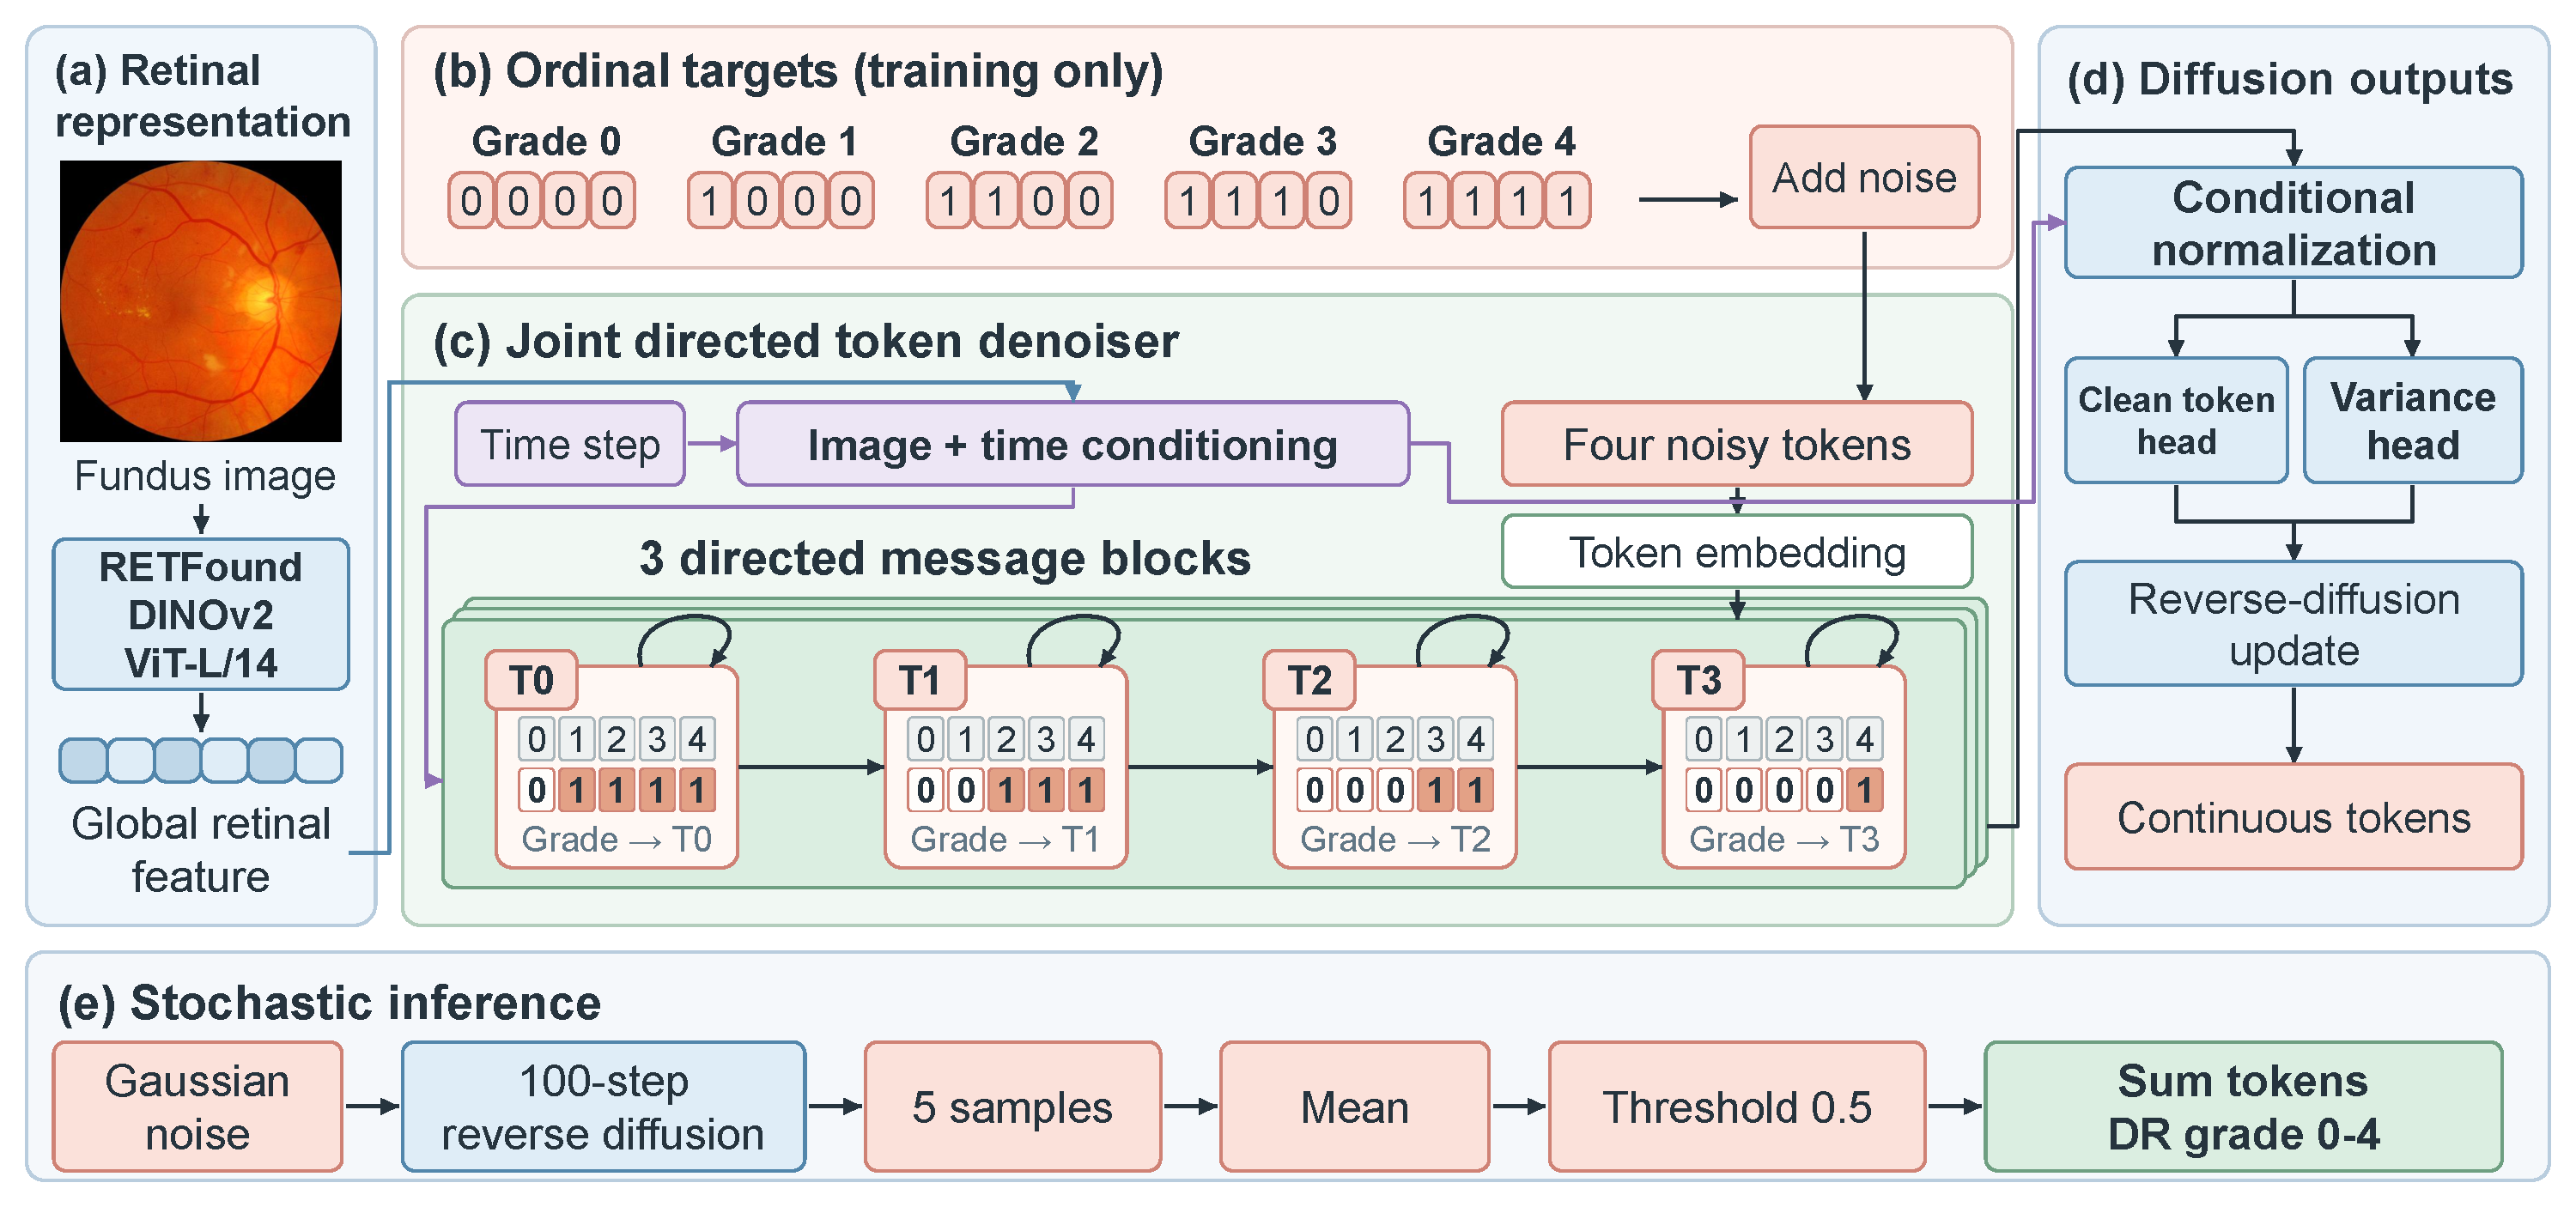
\includegraphics[width=\linewidth]{directed_ordinal_framework_compact_v9_thresholds.pdf}
\caption{Joint directed ordinal-token diffusion. Four cumulative targets define threshold nodes that indicate whether the grade exceeds each boundary. During training, noise is added to these tokens. The conditional denoiser jointly updates all four nodes through three directed message blocks and predicts clean tokens and variance parameters. Inference averages five 100-step samples before thresholding and summation.}
\label{fig:method}
\end{figure}

\subsection{Datasets and preprocessing}

Images and fixed five-grade manifests were taken from the local FundusDG\_mini package organized for GDRBench \citep{che2023gdrnet,gdrbenchguide}. The six training and evaluation manifests for MESSIDOR, APTOS, and DEEPDR are byte-identical to the corresponding upstream GDRBench files. We retain the manifest name MESSIDOR for its MESSIDOR-2 subset. The official MESSIDOR-2 release contains 1748 images but does not supply DR grades \citep{messidor2resource}. After normalizing filename case, all 1744 local image identifiers and grades match the gradable entries in the Google Brain adjudicated five-grade release \citep{googlebraingrades,krause2018reference}. The four remaining entries in that release are marked ungradable and have no DR grade. This metadata correspondence does not verify local image pixels against the original release. \tbc{Confirm the original image-access record and preprocessing chain.}

The available local manifests contain 1744 MESSIDOR, 3662 APTOS, and 2000 DEEPDR records \citep{aptos2019,liu2022deepdrid}. MESSIDOR supports model development, while APTOS and DEEPDR support exploratory transfer analysis. Figure~\ref{fig:distribution} pools the locally available records within each dataset to describe the label distribution. Normal and moderate cases dominate, whereas the severe grades remain sparse, most clearly in MESSIDOR. This descriptive pooling does not alter the fixed partitions used by the experiments. The manifests have not been certified as patient-disjoint.

All 2000 DEEPDR image identifiers and grades match the original DeepDRiD label files. Its local training manifest combines the provider's 1200-image training and 400-image validation sets, while the local evaluation manifest matches the 400-image online challenge evaluation set. The training and validation CSV files provide explicit patient identifiers, but the online grade sheet does not. Filename-prefix separation alone is not treated as verified patient-level separation.

\begin{figure}
\centering
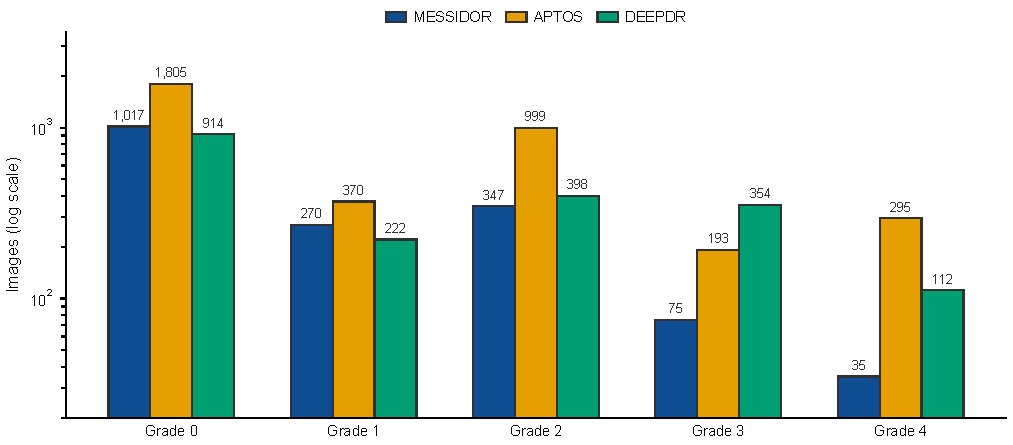
\includegraphics[width=\linewidth]{class_distribution.pdf}
\caption{Pooled grade distributions across the locally available MESSIDOR, APTOS, and DEEPDR manifests. The logarithmic axis shows the concentration of samples in the lower and middle grades and the scarcity of high-severity cases.}
\label{fig:distribution}
\end{figure}

All three sources use the supplied preprocessed image files. GDRBench documents retinal-field extraction and resizing to $512\times512$ pixels \citep{gdrbenchguide}. Our model input pipeline resizes these files to $224\times224$ and applies the ImageNet mean and standard deviation. Training includes random horizontal flipping. Evaluation uses deterministic resizing and normalization, with shuffling disabled. Additional image modification is used only in explicitly identified augmentation experiments.

\subsection{Training, inference, and evaluation protocol}

The RETFound structural comparison uses 50 epochs with AdamW, batch size 64, a constant learning rate of $10^{-4}$, and weight decay 0.01. The historical ViT-B reference was trained for 300 epochs and is not a matched training-budget backbone ablation. Diffusion uses 1000 training steps, a denoiser width of 1024, three denoising blocks, and 100 sampling steps. Each training image contributes four independent diffusion noise draws per call while its encoder representation is reused. This repetition is distinct from the four-token loss multiplier in Eq.~\eqref{eq:diff}. Structural comparisons report the mean and sample standard deviation over three independent training runs. These standard deviations describe training-run variation, not uncertainty over patients.

The fixed 360-image MESSIDOR evaluation manifest was used for per-epoch validation, checkpoint selection, freezing-depth selection, and later development. For each run we reload the checkpoint selected by validation macro-F1 and report all metrics from that same checkpoint under a fixed evaluation random state, five sampling repeats, and a 0.5 token threshold. Reloading provides a reproducible evaluation of the selected checkpoint, not an independent test set. APTOS and DEEPDR results informed later exploratory analyses. All reported results therefore belong to the development and exploratory evaluation protocol, without a separate untouched confirmation cohort.

Evaluation uses a fixed validation order and separate feature fusion for each image. Sensitivity and specificity follow the standard false-negative and false-positive definitions. Repeated diffusion outputs are averaged in continuous space before a single thresholding operation. Accuracy measures overall correctness, macro-F1 gives equal weight to each grade, and quadratic weighted kappa (QWK) accounts for ordinal distance. Per-grade precision and recall show which classes contribute most to false positives and false negatives.

\subsection{Ethics and consent}

This retrospective computational study used publicly distributed, de-identified benchmark images and did not prospectively recruit participants. \tbc{Insert the authors' institution-specific determination of whether ethics review and informed-consent waiver were required, including an approval or exemption identifier where applicable.}

\section{Experiments and results}
\label{sec:results}

\subsection{Comparison with published and internal baselines}

Table~\ref{tab:overall} places the current results alongside the MESSIDOR baselines reported by AOR-DR \citep{yu2025aordr}. The published and current rows follow different data and training protocols and therefore provide context rather than a direct ranking. Within the current protocol, the RETFound configurations provide the closer comparison.

\begin{table}
\centering
\caption{Published and current MESSIDOR results. Published values are taken from the AOR-DR comparison and use its evaluation protocol; QWK was not reported. Current RETFound values are mean $\pm$ sample standard deviation over three runs. Results from different protocols are not directly comparable.}
\label{tab:overall}
\small
\setlength{\tabcolsep}{3.5pt}
\resizebox{\linewidth}{!}{%
\begin{tabular}{lrrr}
\toprule
Method & Accuracy $\uparrow$ & Macro-F1 $\uparrow$ & QWK $\uparrow$ \\
\midrule
\multicolumn{4}{l}{\emph{Published AOR-DR protocol \citep{yu2025aordr}}} \\
ViT-B/16 & 0.639 & 0.419 & n/r \\
CORAL & 0.622 & 0.187 & n/r \\
CORN & 0.622 & 0.186 & n/r \\
PoEs & 0.447 & 0.281 & n/r \\
GoL & 0.608 & 0.338 & n/r \\
Ord2Seq & 0.647 & 0.341 & n/r \\
CLIP-DR & 0.633 & 0.368 & n/r \\
AOR-DR, affine fusion & 0.583 & 0.376 & n/r \\
AOR-DR, cross-attention & 0.625 & 0.451 & n/r \\
\addlinespace
\multicolumn{4}{l}{\emph{Current development protocol}} \\
ViT-B AR (reference) & 0.5389 & 0.3318 & 0.3840 \\
RETFound AR & $0.7380\pm0.0258$ & $0.6947\pm0.0343$ & $0.8117\pm0.0192$ \\
Directed graph (ours) & $\mathbf{0.7463\pm0.0163}$ & $\mathbf{0.7020\pm0.0428}$ & $\mathbf{0.8184\pm0.0243}$ \\
\bottomrule
\end{tabular}}
\end{table}


The flat joint predictor removes serial feedback but does not encode adjacent threshold order. Adding directed messages produced the strongest mean results in the same-backbone comparison and improved macro-F1 over the flat predictor in every repeated run (Table~\ref{tab:main}). This supports combining joint output with explicit ordinal communication in the present architecture. It does not isolate predecessor edges from other parameterization differences.

The ranking against autoregression varied across runs. Training-matched AR feedback further narrowed the difference without repeating checkpoint selection under the revised rule. The graph therefore does not establish a general advantage over autoregressive decoding. Invalid ordinal codes were uncommon for all three predictors and did not explain their performance ordering.

\begin{table}
\centering
\caption{Structural ablation of token prediction under the same RETFound encoder and development protocol. Autoregression is sequential, the parallel MLP predicts all tokens jointly without explicit edges, and the graph combines joint output with directed predecessor messages. Values are mean $\pm$ sample standard deviation over three runs. The flat and graph predictors are not parameter-matched edge ablations.}
\label{tab:main}
\small
\begin{tabular}{lrrr}
\toprule
Method & Accuracy $\uparrow$ & Macro-F1 $\uparrow$ & QWK $\uparrow$ \\
\midrule
Autoregressive & $0.7380\pm0.0258$ & $0.6947\pm0.0343$ & $0.8117\pm0.0192$ \\
Parallel & $0.7435\pm0.0189$ & $0.6680\pm0.0599$ & $0.8128\pm0.0244$ \\
Directed graph & $\mathbf{0.7463\pm0.0163}$ & $\mathbf{0.7020\pm0.0428}$ & $\mathbf{0.8184\pm0.0243}$ \\
\bottomrule
\end{tabular}
\end{table}

\begin{figure}
\centering
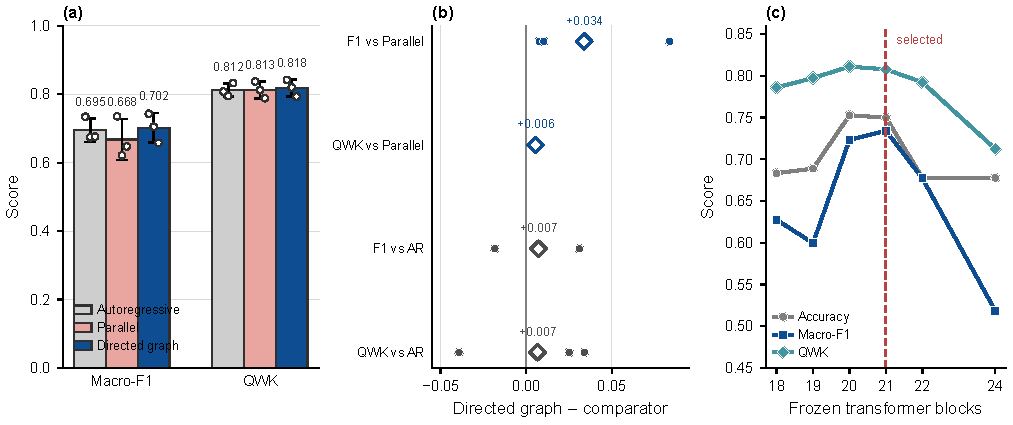
\includegraphics[width=\textwidth]{structure_and_freezing.pdf}
\caption{Token-structure comparison and freezing-depth selection. (a) Mean scores and sample standard deviations over three runs, with circles showing individual runs. (b) Paired differences relative to the directed graph, with diamonds showing mean differences. (c) The RETFound autoregressive freezing-depth screen; each point is one run and the dashed line marks the selected setting.}
\label{fig:structure_freezing}
\end{figure}

\subsection{Retinal representation and freezing depth}

The historical ViT-B runs provide development references with different training histories. Figure~\ref{fig:structure_freezing}(c) shows the RETFound autoregressive freezing-depth experiment. Macro-F1 followed a non-monotonic pattern, with a local decrease at 19 frozen blocks before increasing at 20 and peaking at 21. Since each depth was evaluated once, this variation describes individual runs rather than a causal effect of freezing depth. The 21-block setting was selected using validation macro-F1.

\subsection{Per-grade behavior}

The same-backbone comparison in Table~\ref{tab:pergrade} shows a trade-off across grades. The graph improved mean recall for the two lowest grades, matched autoregression at the middle grade, and performed less well at the two highest grades. Variation across runs and the small number of high-grade cases preclude a claim of uniform improvement. The historical ViT-B result is included only as a reference.

\begin{table}
\centering
\caption{Recall for each MESSIDOR grade. RETFound autoregression (AR) and directed-graph values are mean $\pm$ sample standard deviation over three runs, computed from the unrounded confusion-matrix counts. The ViT-B reference is a single historical run.}
\label{tab:pergrade}
\small
\begin{tabular}{lrrr}
\toprule
Grade & ViT-B reference & RETFound AR & Directed graph \\
\midrule
0 & 0.5982 & $0.8569\pm0.0571$ & $0.8661\pm0.0115$ \\
1 & 0.3774 & $0.3270\pm0.1073$ & $0.3585\pm0.1498$ \\
2 & 0.5775 & $0.6667\pm0.0293$ & $0.6667\pm0.0695$ \\
3 & 0.1667 & $0.7222\pm0.0962$ & $0.6944\pm0.0481$ \\
4 & 0.0000 & $0.9333\pm0.1155$ & $0.8667\pm0.1155$ \\
\bottomrule
\end{tabular}

\end{table}

\subsection{Grade-1 interventions and mechanism-oriented ablations}

Table~\ref{tab:ablation} retains three ablations tied to explicit hypotheses. Grade-1 rebalancing tests whether mild-case exposure is the limiting factor, geometry regularization tests whether an additional ordinal prior is beneficial, and fixed-small variance tests whether the learned sampler variance drives the result. The trained alternatives did not improve balanced recognition and ordinal agreement together. Changing only the sampling variance produced a small class-balanced gain but reduced ordinal agreement. Definitions are given in \ref{app:ablations}.

\begin{table}
\centering
\caption{Hypothesis-driven ablations relative to one directed-graph run. Rebalancing and geometry are separately trained variants. Fixed-small variance changes only inference for the reference checkpoint.}
\label{tab:ablation}
\small
\resizebox{\linewidth}{!}{%
\begin{tabular}{lrrr}
\toprule
Modification & Macro-F1 & QWK & Grade-1 recall \\
\midrule
Directed graph, default & 0.7432 & 0.8418 & 0.5283 \\
Grade-1 rebalancing & 0.6655 & 0.7975 & 0.2642 \\
Geometry regularization & 0.6788 & 0.8129 & 0.3019 \\
Fixed-small inference variance & 0.7476 & 0.8363 & 0.5660 \\
\bottomrule
\end{tabular}}
\end{table}

A separate three-run check of grade-1 rebalancing reached the same conclusion: it did not outperform the unchanged graph on balanced recognition or ordinal agreement. Because the intervention uses only image-level grades, it does not demonstrate improved microaneurysm detection.

\subsection{Exploratory external-domain evaluation}

Transfer without retraining or threshold adjustment was limited (Table~\ref{tab:external}). On APTOS, the model frequently assigned mild cases to grade 2. Ordinal agreement remained stronger than class-balanced recognition, indicating that approximate severity order was preserved while the boundaries among normal, mild, and moderate cases shifted.

The paired DEEPDR evaluation showed the same divergence between metrics. Relative to autoregression, the directed graph improved ordinal agreement and mild-case recall but reduced overall and class-balanced recognition. Many grade-3 images shifted to grade 4. QWK gives partial credit to neighboring predictions, whereas macro-F1 weights recognition of each class equally. Reading the two metrics together reveals boundary shifts that QWK alone can obscure.

\begin{figure}
\centering
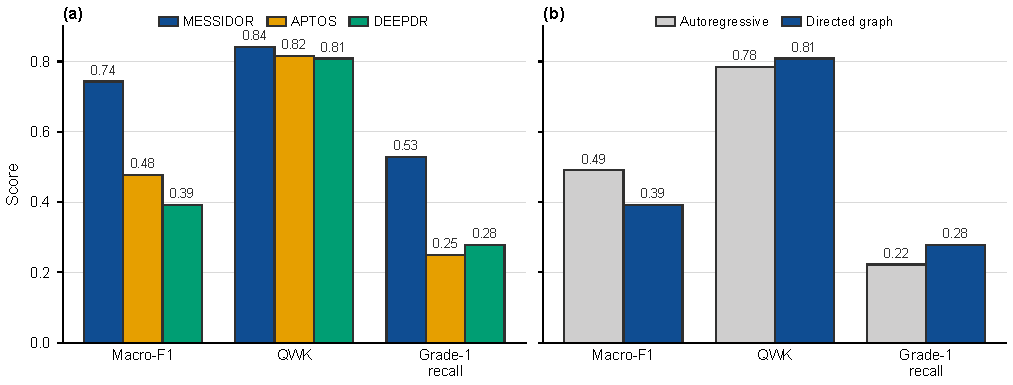
\includegraphics[width=\linewidth]{domain_generalization.pdf}
\caption{External-domain results. Panel (a) compares one fixed directed-graph checkpoint across three datasets. Panel (b) compares autoregressive and directed predictors on DEEPDR. These are single-run exploratory results without uncertainty intervals.}
\label{fig:domain}
\end{figure}

\begin{table}
\centering
\caption{Exploratory transfer of fixed MESSIDOR-trained checkpoints. Macro-F1 measures class-balanced recognition, while QWK tests whether ordinal agreement remains despite shifted grade boundaries.}
\label{tab:external}
\small
\resizebox{\linewidth}{!}{%
\begin{tabular}{llrrr}
\toprule
Dataset & Predictor & Macro-F1 & QWK & Grade-1 recall \\
\midrule
MESSIDOR & Directed graph & 0.7432 & 0.8418 & 0.5283 \\
APTOS & Directed graph & 0.4774 & 0.8165 & 0.2500 \\
DEEPDR & Autoregressive & 0.4903 & 0.7848 & 0.2222 \\
DEEPDR & Directed graph & 0.3916 & 0.8083 & 0.2778 \\
\bottomrule
\end{tabular}}
\end{table}

\subsection{Multi-source training}

Adding 1600 DEEPDR training images did not improve APTOS transfer. A 23-epoch run obtained macro-F1 values of 0.6074 on MESSIDOR and 0.4568 on APTOS. Training for 50 epochs recovered MESSIDOR macro-F1 to 0.7375, whereas APTOS macro-F1 fell to 0.3932 and grade-1 recall to 0.0972. Unweighted pooling fit the mixed training set without learning a stable boundary for the unseen source. A single run cannot establish harm from additional data. It shows that source composition and validation strategy require explicit control.

\subsection{Data integrity and duplicate sensitivity}

The sensitivity analysis used SHA-256 of complete image files to identify byte-identical records. The filtered MESSIDOR evaluation manifest excluded one record overlapping training and one redundant evaluation record, leaving 358 of 360. The APTOS manifest excluded 14 records overlapping its own training manifest, five redundant evaluation records, and four records with conflicting labels, leaving 718 of 741. Conflicting groups were excluded without assigning new diagnostic labels. Since the evaluated single-source model was not trained on APTOS, overlap with APTOS training records is not evidence of training leakage for that model.

Re-evaluating the same graph checkpoint under the filtered protocols changed the metrics only slightly (Table~\ref{tab:dedup}). APTOS grade-1 recall remained low, with 17 of 67 cases recognized. These results concern this fixed model and the identified duplicate records. They do not establish that the ranking among autoregressive, parallel, and graph models is unchanged after filtering. Filtering also changes the assignment of stochastic noise to images, so the metric difference is a protocol sensitivity rather than a causal effect of deleting individual images. File hashes do not identify re-encoded copies, near duplicates, paired eyes, or pretraining overlap.

\begin{table}
\centering
\caption{Fixed-checkpoint sensitivity of the single-source graph to byte-identical file exclusions. Values are original $\rightarrow$ filtered evaluation protocols, without retraining.}
\label{tab:dedup}
\small
\resizebox{\linewidth}{!}{%
\begin{tabular}{llrrrr}
\toprule
Model & Dataset & $N$ & Accuracy & Macro-F1 & QWK \\
\midrule
Single-source graph & MESSIDOR & $360\rightarrow358$ & $0.7583\rightarrow0.7514$ & $0.7432\rightarrow0.7393$ & $0.8418\rightarrow0.8334$ \\
Single-source graph & APTOS & $741\rightarrow718$ & $0.5722\rightarrow0.5780$ & $0.4774\rightarrow0.4742$ & $0.8165\rightarrow0.8182$ \\
\bottomrule
\end{tabular}}
\end{table}

\subsection{Limitations}

The MESSIDOR development cohort contains few high-grade cases. Its repeated use for checkpoint and design selection makes the reported values development estimates. External datasets also informed later analyses and cannot serve as untouched confirmation sets. Verified metadata correspondence does not establish the original image-access chain or patient-disjoint sampling. The MESSIDOR-2 pairing spreadsheet was unavailable in the local package, so cross-partition eye-pair overlap remains unchecked. Independent patient-disjoint validation remains necessary for a confirmatory assessment. The historical ViT-B comparison does not isolate retinal pretraining from other changes, and the RETFound runs do not establish performance under every convergence budget.

The graph and flat predictors differ in parameterization as well as communication. Matched node models with predecessor messages disabled are needed to isolate those messages, and reverse or undirected controls are needed to assess the importance of direction. The AR feedback analysis used fixed historical checkpoints, rather than repeating model selection under a training-matched feedback protocol. Most auxiliary experiments contain one run. Training-run standard deviations do not quantify patient sampling uncertainty, and no statistical superiority over autoregression is established.

Without clinician review, the aggregate metrics cannot determine whether mild-case errors reflect missed pathology, image quality, or uncertain labels. The local-feature experiments leave this ambiguity unresolved. A patch with a high attention score may contain a lesion, a vessel, an illumination change, or an artifact. Further error analysis should stratify cases by measurable image quality and include expert review before adding another lesion-level constraint.

Diffusion also incurs stochastic inference costs relative to a single-pass ordinal head. A complete evaluation should report runtime and calibration alongside macro-F1, QWK, and per-grade recall. Clinical claims require patient-disjoint external validation.

\section{Conclusion}
\label{sec:conclusion}

We evaluated a directed ordinal-token graph that jointly predicts clean cumulative tokens within a diffusion sampler. Under a common RETFound development protocol, the graph was stronger than the flat joint predictor and remained close to the autoregressive implementation. The structural ablation suggests that joint output benefits from explicit ordinal communication, but it does not isolate predecessor edges from other parameterization differences or establish superiority over autoregression. Mild-case recognition and transfer across datasets remain the main weaknesses. Matched edge ablations, verified dataset provenance, and independent patient-disjoint evaluation are required before drawing broader conclusions about reliable DR grading.

\section*{CRediT authorship contribution statement}
\tbc{List every author and verified CRediT role. Do not infer roles from author order.}

\section*{Declaration of competing interest}
\tbc{Insert the verified competing-interest statement and complete the journal's separate declaration workflow.}

\section*{Data availability}
Source dataset access points are the \href{https://www.adcis.net/en/third-party/messidor2/}{MESSIDOR-2 resource}, the \href{https://www.kaggle.com/competitions/aptos2019-blindness-detection}{APTOS competition}, and the \href{https://github.com/deepdrdoc/DeepDRiD}{DeepDRiD repository}. MESSIDOR-2 grade metadata are available from the \href{https://www.kaggle.com/datasets/google-brain/messidor2-dr-grades}{Google Brain annotation release}. Benchmark preparation is documented in the \href{https://github.com/chehx/DGDR/tree/main/GDRBench}{GDRBench guide}. Local manifests, rather than official dataset-wide counts, define the samples used here. Metadata were checked against these sources on 16 October 2026. The ADCIS image-access conditions are separate from the annotation release and the local mirror's license metadata. \tbc{Confirm the original image-access records and applicable conditions, and the availability of code, exact splits, pretrained-checkpoint identifiers, trained weights, and per-image predictions. No public code deposit is asserted in this draft.}

\section*{Acknowledgements}
\tbc{Insert verified funding and acknowledgements, or remove this section if none apply.}

\appendix
\section{Definitions of exploratory ablations}
\label{app:ablations}

\paragraph{Grade-1 sampling}
Sampling weights are two for grade-1 images and one for all other grades. Sampling is with replacement, with the number of draws per epoch equal to the size of the original training manifest. The dataset files and labels are unchanged. This changes expected class exposure, rather than doubling the epoch length.

\paragraph{Rank geometry}
Five trainable anchors $\mathbf a_y$ and global retinal features $\mathbf z$ are normalized to unit length. For interior grades 1--3, an order term uses two direction logits given by the feature dot products with the normalized preceding and following anchor differences, multiplied by 20. Cross-entropy selects the following direction. The metric loss is the batch mean of $[m+\|\mathbf{z}-\mathbf{a}_y\|_2-\|\mathbf{z}-\mathbf{a}_{n(y)}\|_2]_+$, where $n(y)=y+1$ for $y<4$ and $n(4)=3$. The margin starts at 0.3 and follows an exponential moving average with coefficient 0.9 of 0.4 times within-class dispersion, averaged over feature coordinates and eligible classes. Dispersion is the population standard deviation of normalized feature coordinates, using only classes with at least two samples in the batch. The total loss is $\mathcal{L}_{\mathrm{joint}}+0.1(\mathcal{L}_{\mathrm{order}}+\mathcal{L}_{\mathrm{metric}})$. The auxiliary terms use each original image once and are absent at inference. This is a component adaptation, not a reproduction of the full DiffGeo-AOR method.

\paragraph{Fixed-small inference variance}
The same trained graph checkpoint and clean-token prediction are retained. During reverse sampling, the posterior small variance replaces the learned variance. This changes the sampler only. Results use the same number of repeats, sampling steps, and threshold as the reference evaluation.

\paragraph{AR feedback sensitivity}
The three historical AR confusion matrices were reproduced exactly. At each fixed checkpoint, the historical and training-matched feedback rules were compared after restoring the same post-initialization Python, NumPy, CPU, and CUDA random states. Final grades changed for 0, 1, and 6 of 360 images across the three checkpoints. Mean macro-F1 changed from $0.6947\pm0.0343$ to $0.7008\pm0.0322$, while QWK changed from $0.8117\pm0.0192$ to $0.8114\pm0.0197$. Mean grade-1 recall decreased from $0.3270\pm0.1073$ to $0.3208\pm0.0998$. One corrected grade-4 prediction contributed to the largest single-run macro-F1 increase, illustrating sensitivity to the five available grade-4 cases. The results do not support feedback conversion as a remedy for mild-case recognition in this protocol.

\bibliographystyle{cas-model2-names}
\bibliography{references}
\end{document}
